\documentclass[12pt]{article}
\usepackage{fullpage,graphicx,amsmath,amsfonts,forest,listings,xcolor}
\usepackage[hidelinks]{hyperref}
\usepackage[small,bf]{caption}

\definecolor{bgcolor}{rgb}{0.95,0.95,0.95}
\lstdefinestyle{mystyle}{
basicstyle=\footnotesize\ttfamily,
backgroundcolor=\color{bgcolor},
keywordstyle=\color{violet},
stringstyle=\color{red},
showstringspaces=false,
numbers=left,
frame=line
}
\lstset{
style=mystyle,
breaklines=true,
postbreak=\mbox{\textcolor{red}{$\hookrightarrow$}\space}
}

\input defs.tex

\bibliographystyle{alpha}

\title{
Programming Assignments 2: Java Parser \\
\large CSE360, Design and Implementation of Compiler
}
\author{
Shao-Hsuan Chu \\
Instructor: Ye-In Chang \\
Teaching Assistant: Sheng-Hsin Chiang \\
\\
National Sun Yat-sen University
}

\begin{document}
\maketitle
\newpage

\tableofcontents
\newpage

\section{Introduction}
In this assignment, we're required to implement a syntactic parser for Java programming language in Lex \& Yacc. The parser need to have three main features below.

\begin{itemize}
    \item A scanner to correctly extract tokens from the raw input and pass them onto the next stage. It also has to identify the redundant characters if they cannot be recognized as any token.
    \item A parser to examine the syntactic structure based on a pre-defined Java grammar. Upon encountering an error, it needs to be able to recover and keep parsing the rest of the input source file. An expressive error message is also preferred.
    \item A simple semantic check for redefinitions in the same scope and unused variables.
\end{itemize}

\section{File structure}

\begin{forest}
for tree={
font=\ttfamily,
grow'=0,
child anchor=west,
parent anchor=south,
anchor=west,
calign=first,
edge path={
\noexpand\path [draw, \forestoption{edge}]
(!u.south west) +(7.5pt,0) |- node[fill,inner sep=1.25pt] {} (.child anchor)\forestoption{edge label};
},
before typesetting nodes={
if n=1
{insert before={[,phantom]}}
{}
},
fit=band,
before computing xy={l=50pt},
}
[.
    [README.pdf]
    [TestingFiles
	[test1-6.java]
    ]
    [src
	[Scanner.l]
	[Parser.y]
	[Makefile]
	[SymbleTable
	    [SymbolTable.c]
	    [SymbolTable.h]
	]
	[utils
	    [ListOptionals.sh]
	    [ListTokens.sh]
	]
    ]
]
\end{forest}

\begin{itemize}
    \item \texttt{README.pdf}: This file
    \item \texttt{TestFiles}
    \begin{itemize}
	\item \texttt{test1-6.java}: six testing files
    \end{itemize}
    \item \texttt{src}: source code
    \begin{itemize}
	\item \texttt{Scanner.l}: Lex code
	\item \texttt{Parser.y}: Yacc code
	\item \texttt{Makefile}: Compile Lex, Yacc and C source code
	\item \texttt{SymbolTable}: Symbol table header and implementation using hash table
	\item \texttt{utils}: Utilities
	\begin{itemize}
	    \item \texttt{ListOptionals.sh}: Take Lex source file and extract the tokens after the keyword \texttt{return} and removes the duplicates.
	    \item \texttt{ListTokens.sh}: Take Yacc source file and extract all of the optionals then generates the rules for them.
	\end{itemize}
    \end{itemize}
\end{itemize}

\section{Environment}
\subsection{Operating systems}
\begin{itemize}
    \item macOS 11.4
    \item Ubuntu 18.04.5 LTS
\end{itemize}
\subsection{Lex compiler}
\begin{itemize}
    \item flex 2.5.35 Apple(flex-32)
    \item flex 2.6.4
\end{itemize}
\subsection{Yacc compiler}
\begin{itemize}
    \item bison (GNU Bison) 2.3
    \item bison (GNU Bison) 3.0.4
\end{itemize}

\section{Usage}
\subsection{Build}
To build the \texttt{JavaParser} from source, use \texttt{make}.

\begin{lstlisting}[language=sh]
cd src
make [DEBUG=<level>]
\end{lstlisting}

where you can set the optional flag \texttt{DEBUG} to a desired level. If the flag is not provided, then it defaults to level \texttt{0}.
\subsection{Debugging level}
The available levels include:

\begin{itemize}
    \item \texttt{Level 0}: Print the errors and warnings only.
    \item \texttt{Level 1}: Print the original source code and errors/warnings in the context.
    \item \texttt{Level 2}: Same as above but this one also prints the symbol table.
    \item \texttt{Level 3}: In addition to above, this also prints the entire parsing process. This sets \texttt{yydebug} to \texttt{1} in the Yacc source file and generate \texttt{y.output}, which contains all of the states and rules.
\end{itemize}

\subsection{Execute}
To parse a Java source file, redirect the content into the program. The \texttt{TestingFiles} directory contains six testing files. To test a single file
\begin{lstlisting}[language=sh]
./JavaParser < ../TestingFiles/test1.java
\end{lstlisting}
to test all files altogether
\begin{lstlisting}[language=sh]
cat ../TestingFiles/* | ./JavaParser
\end{lstlisting}



\section{Implementation}
\subsection{Lexical analysis}

Despite the Java's capability of allowing Unicode characters, only ASCII characters can be accepted by the parser in this work for the sake of simplicity. In lexical analysis, the mission is to combine one or more characters in to various tokens. The tokens can be divided into three main groups which are \texttt{literals}, \texttt{keywords \& operators} and \texttt{identifier \& others}. 

\subsubsection{Literals}

There are six kinds of literals in Java. They are

\paragraph{Boolean literal.}
For the boolean literal, the accepted words can be either \texttt{true} or \texttt{false}.
\paragraph{Null literal.}
For the null literal, it just accepts \texttt{null}.
\paragraph{Character literal.}
For the character literal, the content must be included in two single quotes and it accept any character except \texttt{single quote}, \texttt{new line character}, and \texttt{backslash}. However, the escape sequence is also accepted by the content. See the following Lex source code.
\lstinputlisting[linerange={23-24}]{../src/Scanner.l}
\paragraph{String literal.}
For the string literal, the content must be included in two double quotes and it accept any characters except \texttt{double quotes}, \texttt{new line characters}, and \texttt{backslashes}. However, the escape sequence is also accepted by the content. See the following Lex source code.
\lstinputlisting[linerange={25-25}]{../src/Scanner.l}
\paragraph{Integer literal.}
The integer literal can be further decomposed into \texttt{decimal}, \texttt{hexadecimal} and \texttt{octal} integer literals with a shared optional postfix \texttt{l} or \texttt{L}. See the following Lex source code.
\lstinputlisting[linerange={27-31}]{../src/Scanner.l}
\paragraph{Floating-point literal.}
The floating-point literal accepts the integer literal plus \texttt{decimal point} and \texttt{scientific notation} with an optional postfix \texttt{f} or \texttt{F} for single-precision floating-point and \texttt{d} or \texttt{D} for the double-precision one.
\lstinputlisting[linerange={33-33}]{../src/Scanner.l}

\subsubsection{Keywords \& Operators}
\paragraph{Keywords}
The keywords in Java is reserved. Defining them before the identifier prevents the word from being matched with the identifier token. Here's a list of keywords in the original Java. Noted that \texttt{const} and \texttt{goto} are keywords but never used in Java, hence none of the productions in the next stage use them. Consequently, we don't have to pass them as tokens onto the next stage of parsing.
\begin{lstlisting}[language=Java]
abstract boolean break byte case catch char class const continue default 
do double else extends final finally float for goto if implements import 
instanceof int interface long native new package private protected public
return short static super switch synchronized this throw throws transient
try void volatile while
\end{lstlisting}
\paragraph{Operators}
We also need to capture the operators one by one and pass them as tokens onto the next stage. Here's a list of operators in Java.
\begin{lstlisting}[language=Java]
= *= /= %= += -= <<= >>= >>>= &= ^= |= << >> >>> == != <= >= < > && || ! ++ -- & | ^ ~ * / % + - ? : . { } [ ] ( ) , ;
\end{lstlisting}

\subsubsection{Identifier \& Others}
\paragraph{Identifier}
The identifier in Java can start with any Unicode characters except digits and some symbols. However, as mentioned above, only ASCII characters are allowed in this work. As the regular expression goes
\lstinputlisting[linerange={35-35}]{../src/Scanner.l}

\paragraph{Others}
Other tokens include \texttt{space}, \texttt{new line character} and \texttt{comment}. There are recognized so they won't be redundant characters, but they won't be passed onto the next stage, either. The space includes single space characters and tabular characters while the comment allows both C-style (/* */) and C++-style (//) comments. See the regular expressions below.

\lstinputlisting[linerange={36-37}]{../src/Scanner.l}

\subsection{Syntax analysis}
To maximize the power or error detection in Yacc, I've tried to minimize the use of Lex so the parser can identify the error at a critical state. This enables the parser to generate expressive error message instead of only indicating the redundant characters. Still, as mentioned above, the literals were packed into an atomic token in the lexical analysis stage. This prevents, for example, a floating-point prefix \texttt{f} (as in \texttt{float foo = 1.1f;}) from being recognized as an identifier \texttt{f} (as in \texttt{int f;}).

\subsubsection{From BNF to LALR(1)}
When writing production rules, in addition to follow the given Java grammar, extra modification must also be made. Since Yacc is an LALR(1) parser, a Backus normal form (BNF) grammar cannot be directly applied to our implementation. There are five problems if we want to use Java BNF grammar in Yacc.
\paragraph{1. Ambiguous names.}
Look at a snippet in the original Java BNF grammar.

\lstinputlisting{BNFtoLALR/Problem1.m}

Now, consider the input

\begin{lstlisting}[language=Java]
class foo { int f() { whichami.
\end{lstlisting}

When the parser is considering the token \texttt{whichami}, with one token lookahead to \texttt{.} (the dot), it cannot tell whether \texttt{whichami} is a \texttt{package name} that qualifies a \texttt{type name}, as in

\begin{lstlisting}[language=Java]
class foo { int f() { whichami.type newOBJ; }
\end{lstlisting}

Or a \texttt{ambiguous name} that qualifies a \texttt{method name}, as in

\begin{lstlisting}[language=Java]
class foo { int f() { whichami.method(); }
\end{lstlisting}

\subparagraph{Solution.} We can replace \texttt{PackageName}, \texttt{TypeName}, \texttt{ExpressionName}, \texttt{MethodName}, and \texttt{AmbiguousName} with an single nonterminal \texttt{Name}.

\lstinputlisting[linerange={122-128}]{../src/Parser.y}

And a later stage of compiler analysis would figure it out the precise role or the names. In other words, this cannot be determinant in the parsing stage.

\paragraph{2. Various sets of modifiers.}
Look at a snippet in the original Java BNF grammar.
\lstinputlisting{BNFtoLALR/Problem2.m}
The problem is similar to the problem 1, the parser may not be able to determine whether it should reduce the token to a \texttt{field declaration} or a \texttt{method declaration}. Plus, since the number of modifiers can be zero to infinite, a lookahead-1 parser can never make a decision based on the next token.
\subparagraph{Solution.} Same as above, we delay the decision which set of modifiers should be applied to the later stage of analysis. Again, in other words, the parser cannot determine which set of modifiers is allowed.

\paragraph{3. Field declaration versus method declaration.}
After we merged various sets of modifiers into one unique token, the parser still cannot determine whether it is a \texttt{field declaration} or a \texttt{method declaration}. Consider the input

\begin{lstlisting}[language=Java]
class foo { int whichami
\end{lstlisting}
When the parser is considering the token \texttt{int}, with one token lookahead to \texttt{whichami}, it cannot tell whether the following input would be which one of the following
\begin{lstlisting}[language=Java]
class foo { int whichami = 0; }

class foo { int whichami(int arg); }
\end{lstlisting}
And shifts the \texttt{int} or reduce it to \texttt{ResultType}, respectively.

\subparagraph{Solution.} we can eliminate the \texttt{ResultType} production and have separate alternatives of \texttt{Type} and \texttt{void}.

\lstinputlisting[linerange={229-229,242-242,255-255}]{../src/Parser.y}

So the parser can proceed to consider \texttt{whichami}, with one token lookahead to \texttt{=} or \texttt{(}, hence being determinant.

\paragraph{4. Array type or access.}
Look at a snippet in the original Java BNF grammar.
\lstinputlisting{BNFtoLALR/Problem4.m}
Now, consider the input
\begin{lstlisting}[language=Java]
class foo { foo() { whichami[
\end{lstlisting}
The parser is now considering \texttt{whichami}, with one token lookahead to \texttt{[}. It cannot determine whether this is a variable declaration with type of \texttt{whichami[]}, as in
\begin{lstlisting}[language=Java]
class foo { foo() { whichami[] var; } }
\end{lstlisting}
Or an array access, as in
\begin{lstlisting}[language=Java]
class foo { foo() { whichami[0] = 1; } }
\end{lstlisting}

\subparagraph{Solution.} we should separate alternatives for \texttt{ArrayType}

\lstinputlisting[linerange={116-119}]{../src/Parser.y}

So the parser can reduce \texttt{whichami} to \texttt{Name} and proceed to consider \texttt{[}, with one token lookahead to \texttt{]} or \texttt{0}, hence being determinant.

\paragraph{5. Cast versus parenthesized expression.}
The corresponding grammar
\lstinputlisting{BNFtoLALR/Problem5.m}
Consider the following input
\begin{lstlisting}[language=Java]
class foo { foo() { super((whichami)
\end{lstlisting}
Supposed the parser is considering \texttt{whichami}, with one token lookahead to \texttt{)}. The ambiguity lies between
\begin{lstlisting}[language=Java]
class foo { foo() { super((whichami)); }

class foo { foo() { super((whichami)toBeCasted); }
\end{lstlisting}
Although few people would parenthesize a single variable, but it is legal. Therefore, the parser cannot decide which one above to take.

\subparagraph{Solution.} The solution is to eliminate the use of the nonterminal \texttt{ReferenceType} in the definition of \texttt{CastExpression}, which requires some reworking of both alternatives to avoid other ambiguities
\lstinputlisting[linerange={531-534}]{../src/Parser.y}

\subsubsection{Precedence \& Associativity}
Specifying the precedence and the associativity among operators is crucial for eliminating shift-reduce conflict. Following the Java's specification, the associativity can be specified by \texttt{\%right}, \texttt{\%left} or \texttt{\%nonassoc} in the Yacc source file as below.
\lstinputlisting[linerange={49-64}]{../src/Parser.y}
where the precedence is implied in the order of these lines. The latter an associativity rule is specified, the higher precedence the operators get.

Typically, the precedence of a production is determined by the last terminal's precedence. However, in some cases, the terminal itself is insufficient to expressive the proper precedence. For example, the \texttt{-} operator in the production of an unary expression, i.e., \texttt{-} as a negative sign instead of a subtraction operator. At this point, the precedence of the subtration operator is insufficient to express the one for an unary expression, so we can use \texttt{\%prec} followed by a flag defined above, which should be \texttt{UMINUS} in this case. This technique can also be applied to postfix and prefix increment/decrement operators with shared tokens \texttt{++}/\texttt{--}.
\lstinputlisting[linerange={512-525}]{../src/Parser.y}
\subsubsection{Optionals}
As we would've seen the optional symbols in the Java grammar, which are followed by the question mark \texttt{?}. We will not be able to directly use that notation in the implementation in Yacc since there's no such feature. Instead, in this work, all of the optionals are marked with the prefix of \texttt{Opt}, which can be identify by the script \texttt{ListOptionals.sh} as listed in the section 2.
\lstinputlisting[language=sh]{../src/utils/ListOptionals.sh}
This shell script finds all optionals and generates the corresponding production for each.
\lstinputlisting[linerange={600-619}]{../src/Parser.y}

\subsection{Semantic analysis}
The semantic analysis in this work only provides two simple checks, redefinition in the scope and unused variables.
\subsubsection{Redefinition check}
The redefinition check can be achieved by the help of a well-designed symbol table. In this work, the scope is recorded by a stack, and each scope has its own dedicated symbol table. The structure can be found in the header file \texttt{SymbolTable.h}.
\lstinputlisting[linerange={40-63}]{../src/SymbolTable/SymbolTable.h}
\subsubsection{Unused variable check}
In order to track the number or access to a symbol, we need to add a column \texttt{Occurrence} in each entry in the symbol table. The \texttt{Occurrence} only increments when a local variable is accessed, e.g., in an expression or at the left-hand side of an assignment statement. Only the method-like blocks are being examined in this work, i.e., the field in a class declaration would not be taken into account.

\section{Screenshots}
\newpage

\begin{figure}
\begin{center}
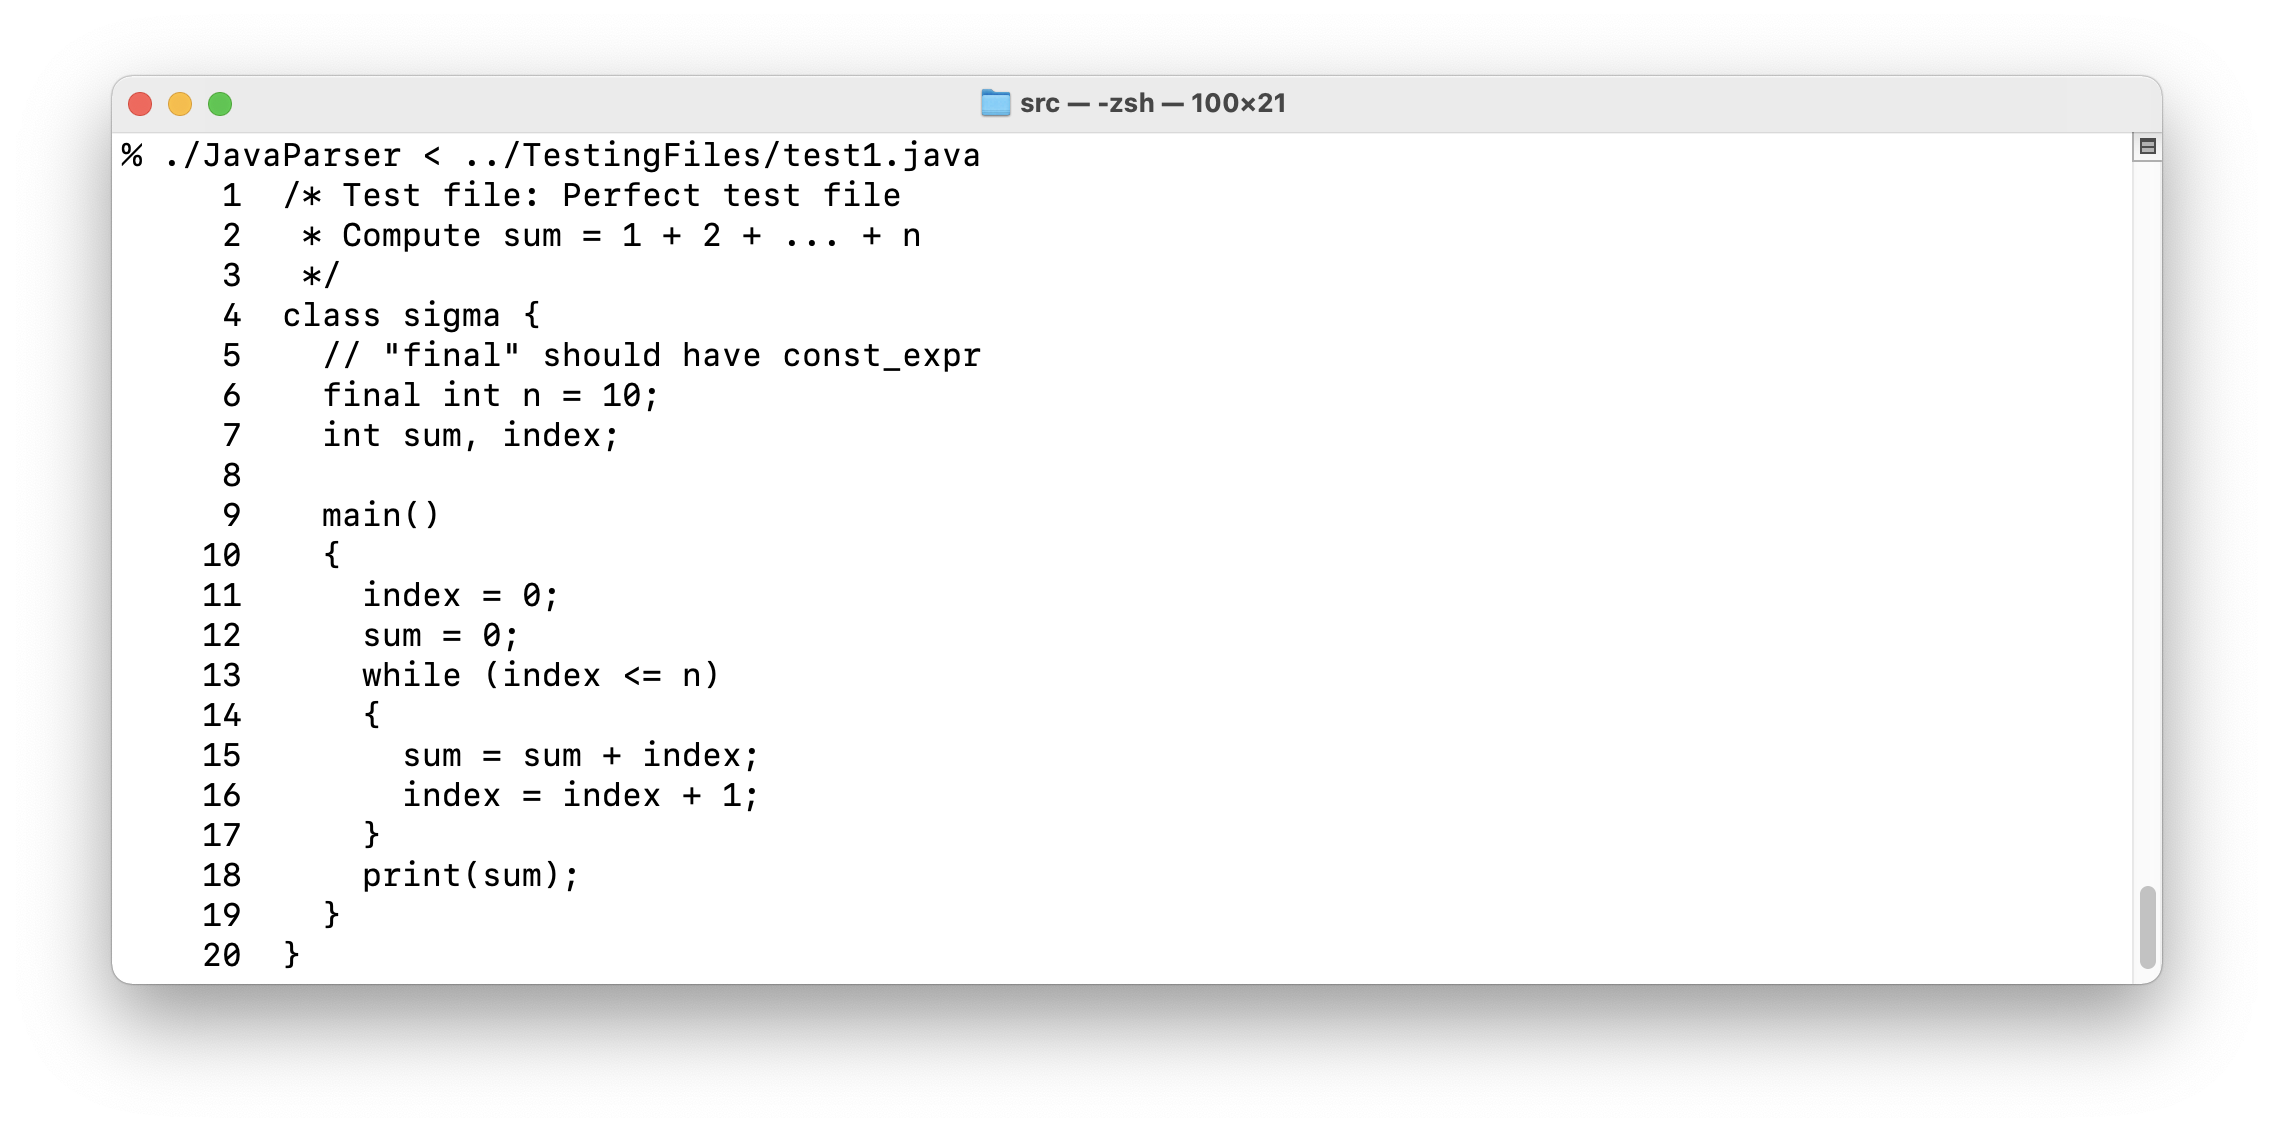
\includegraphics[width=0.9\textwidth]{Screenshots/test1}
\end{center}
\caption{The output of parsing \texttt{test1.java} with \texttt{DEBUG=1}}
\label{test1}
\end{figure}
\begin{figure}
\begin{center}
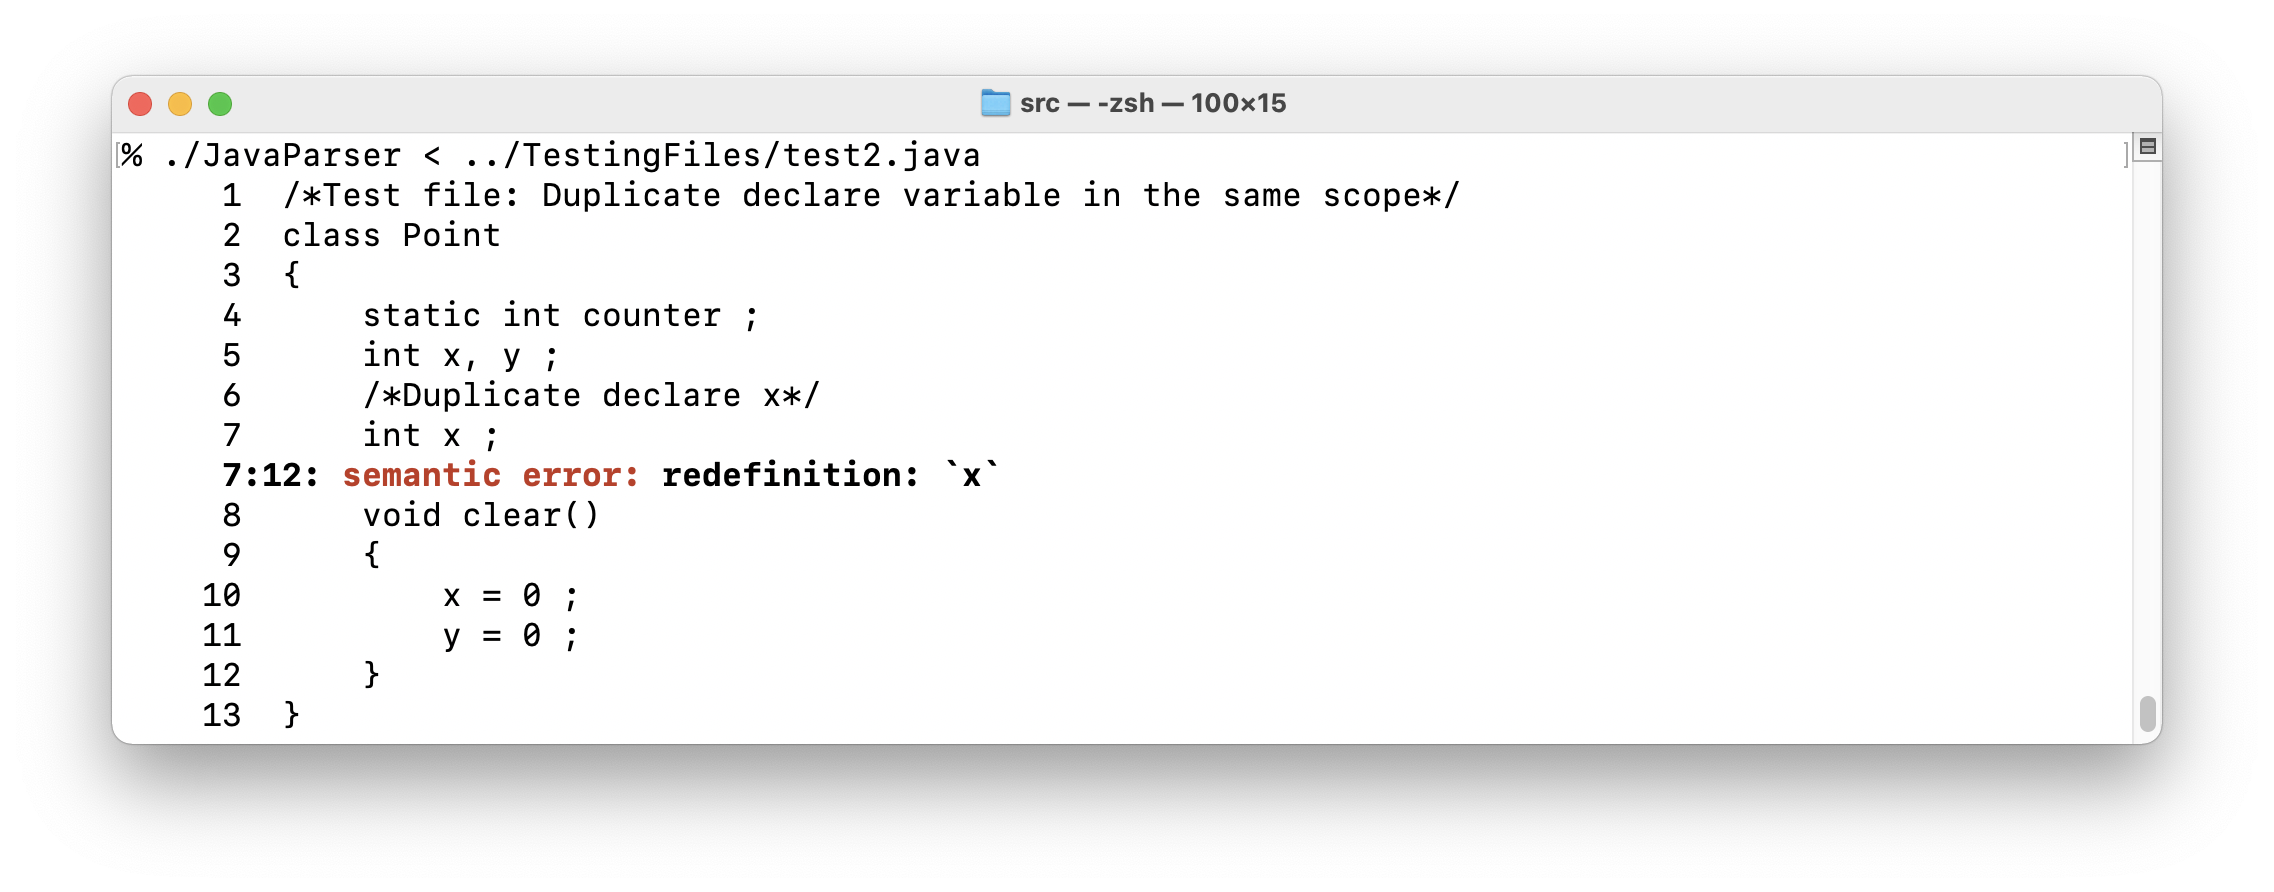
\includegraphics[width=0.9\textwidth]{Screenshots/test2}
\end{center}
\caption{The output of parsing \texttt{test2.java} with \texttt{DEBUG=1}}
\label{test1}
\end{figure}
\begin{figure}
\begin{center}
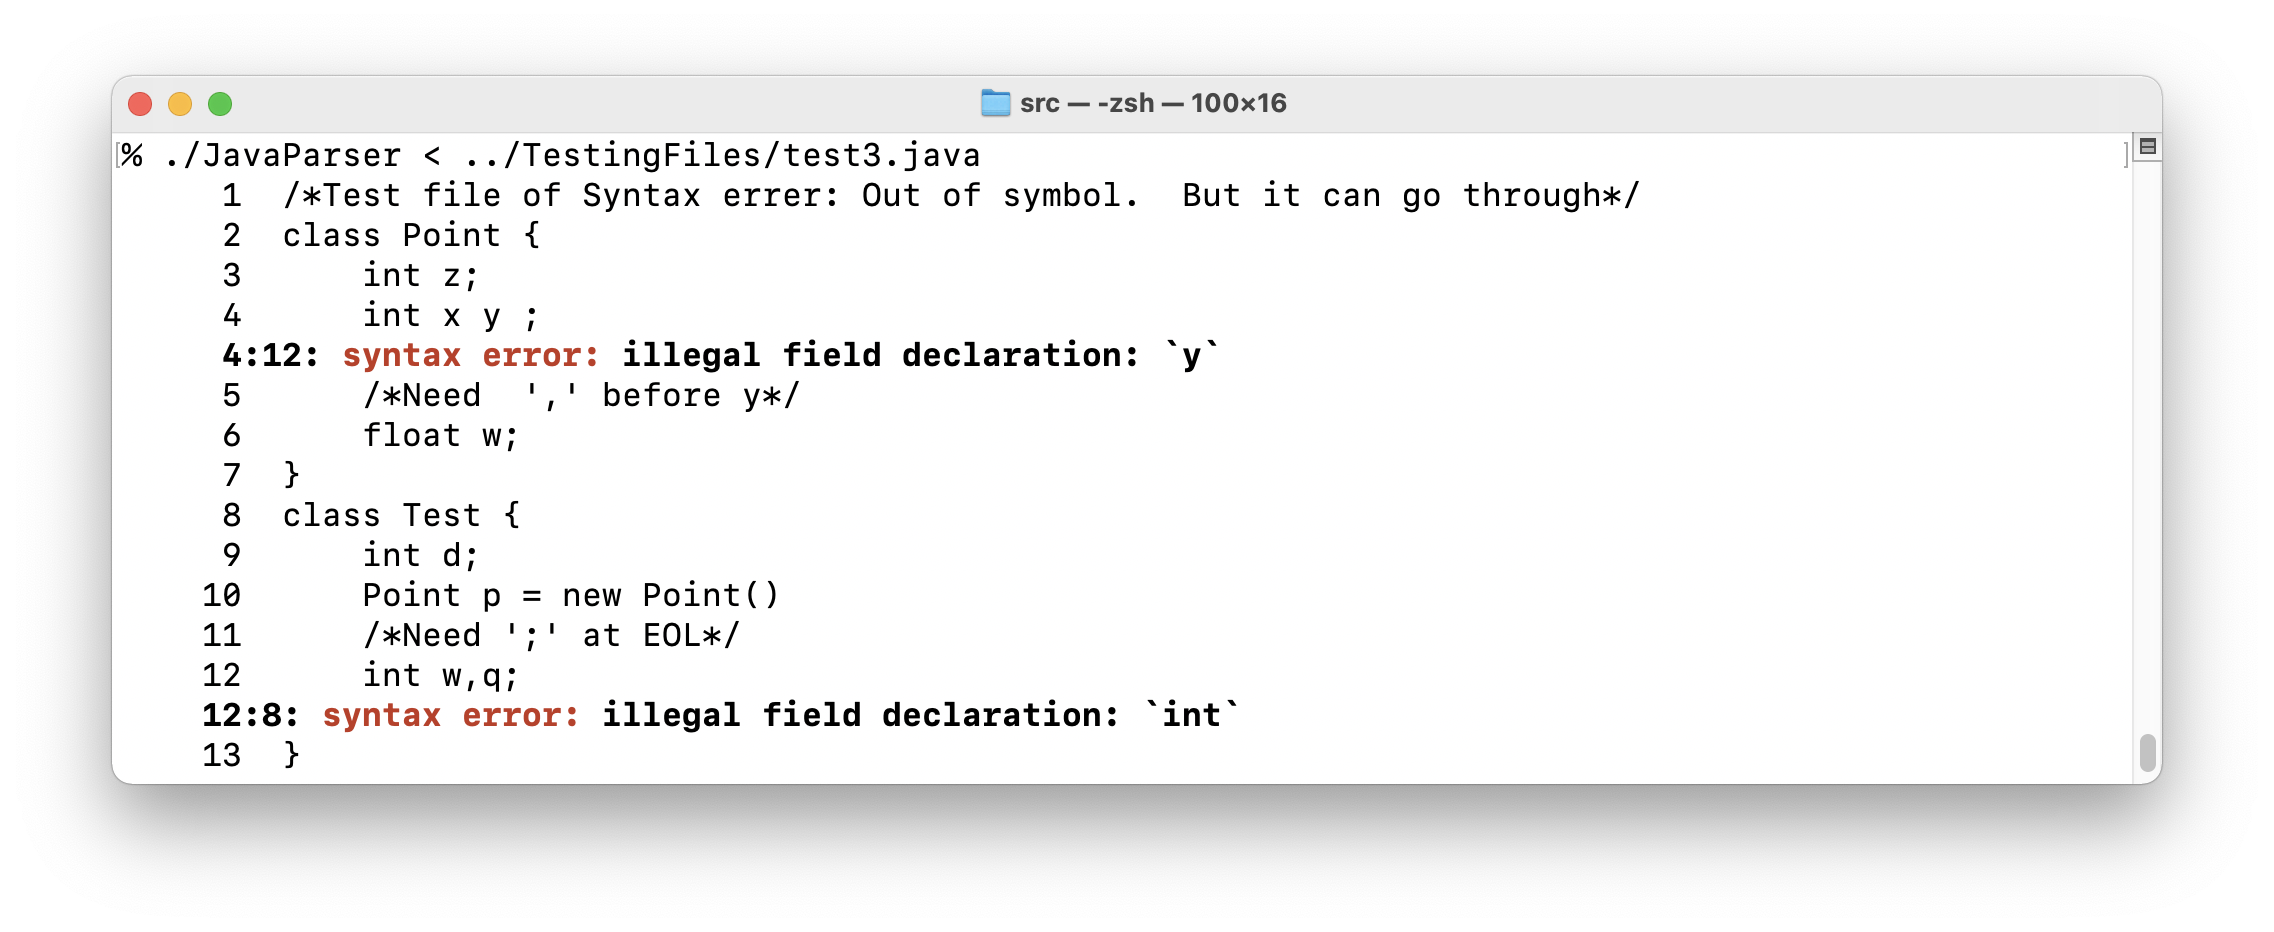
\includegraphics[width=0.9\textwidth]{Screenshots/test3}
\end{center}
\caption{The output of parsing \texttt{test3.java} with \texttt{DEBUG=1}}
\label{test1}
\end{figure}
\begin{figure}
\begin{center}
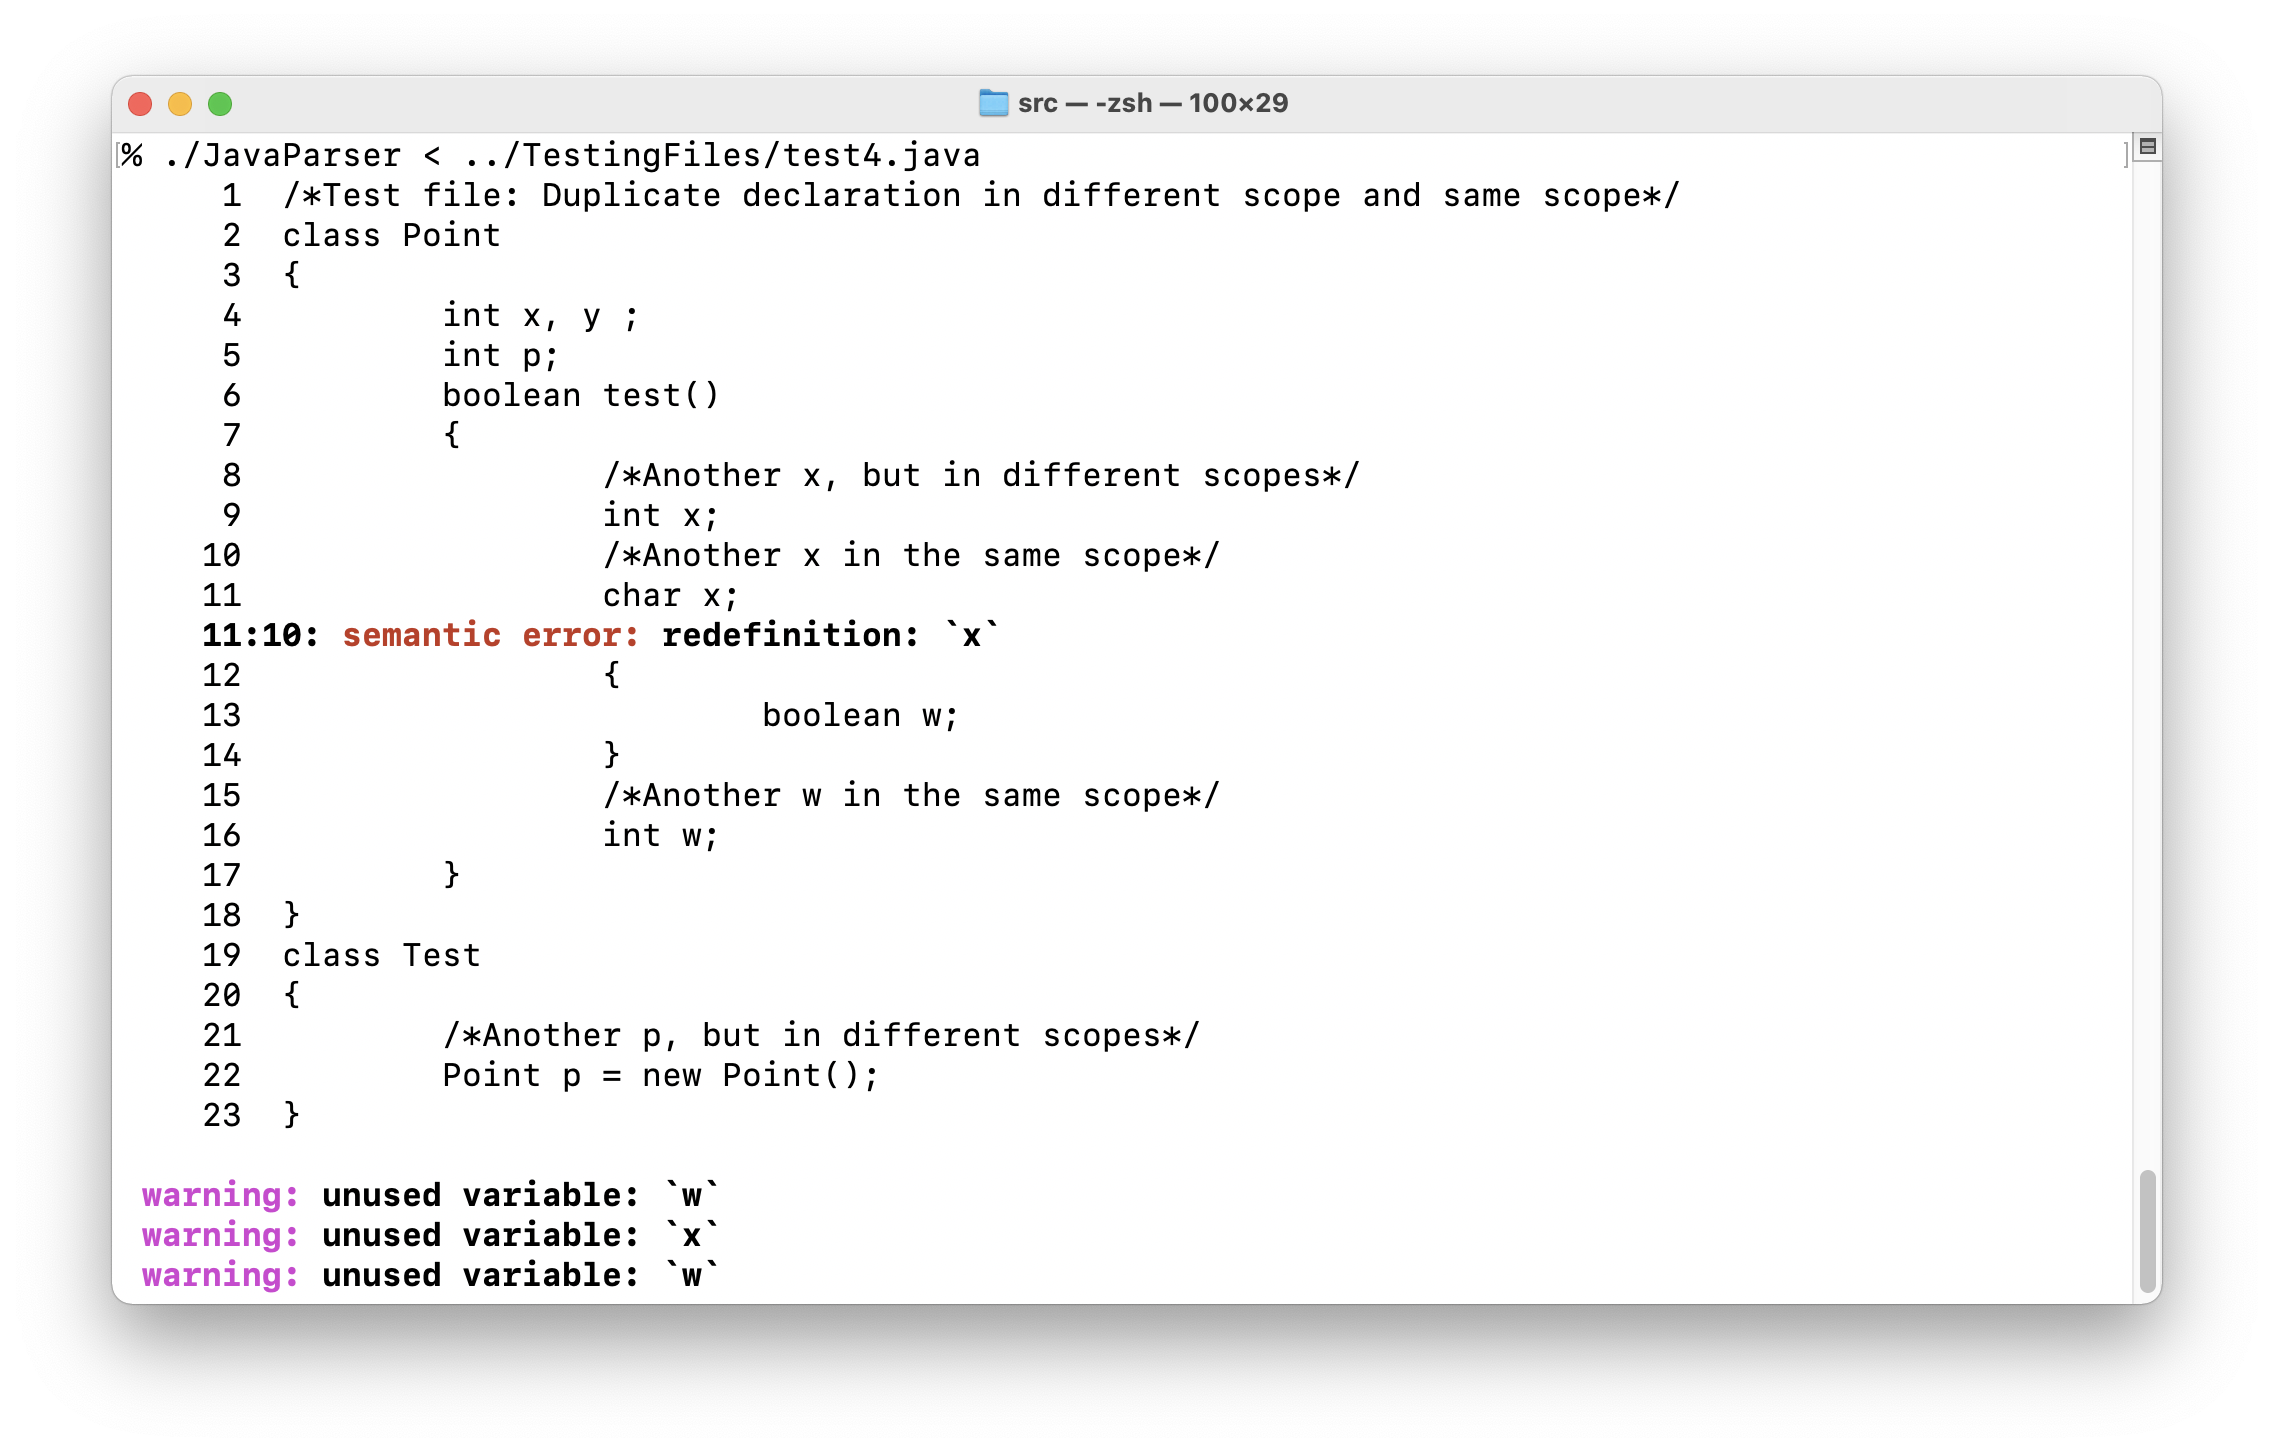
\includegraphics[width=0.9\textwidth]{Screenshots/test4}
\end{center}
\caption{The output of parsing \texttt{test4.java} with \texttt{DEBUG=1}}
\label{test1}
\end{figure}
\begin{figure}
\begin{center}
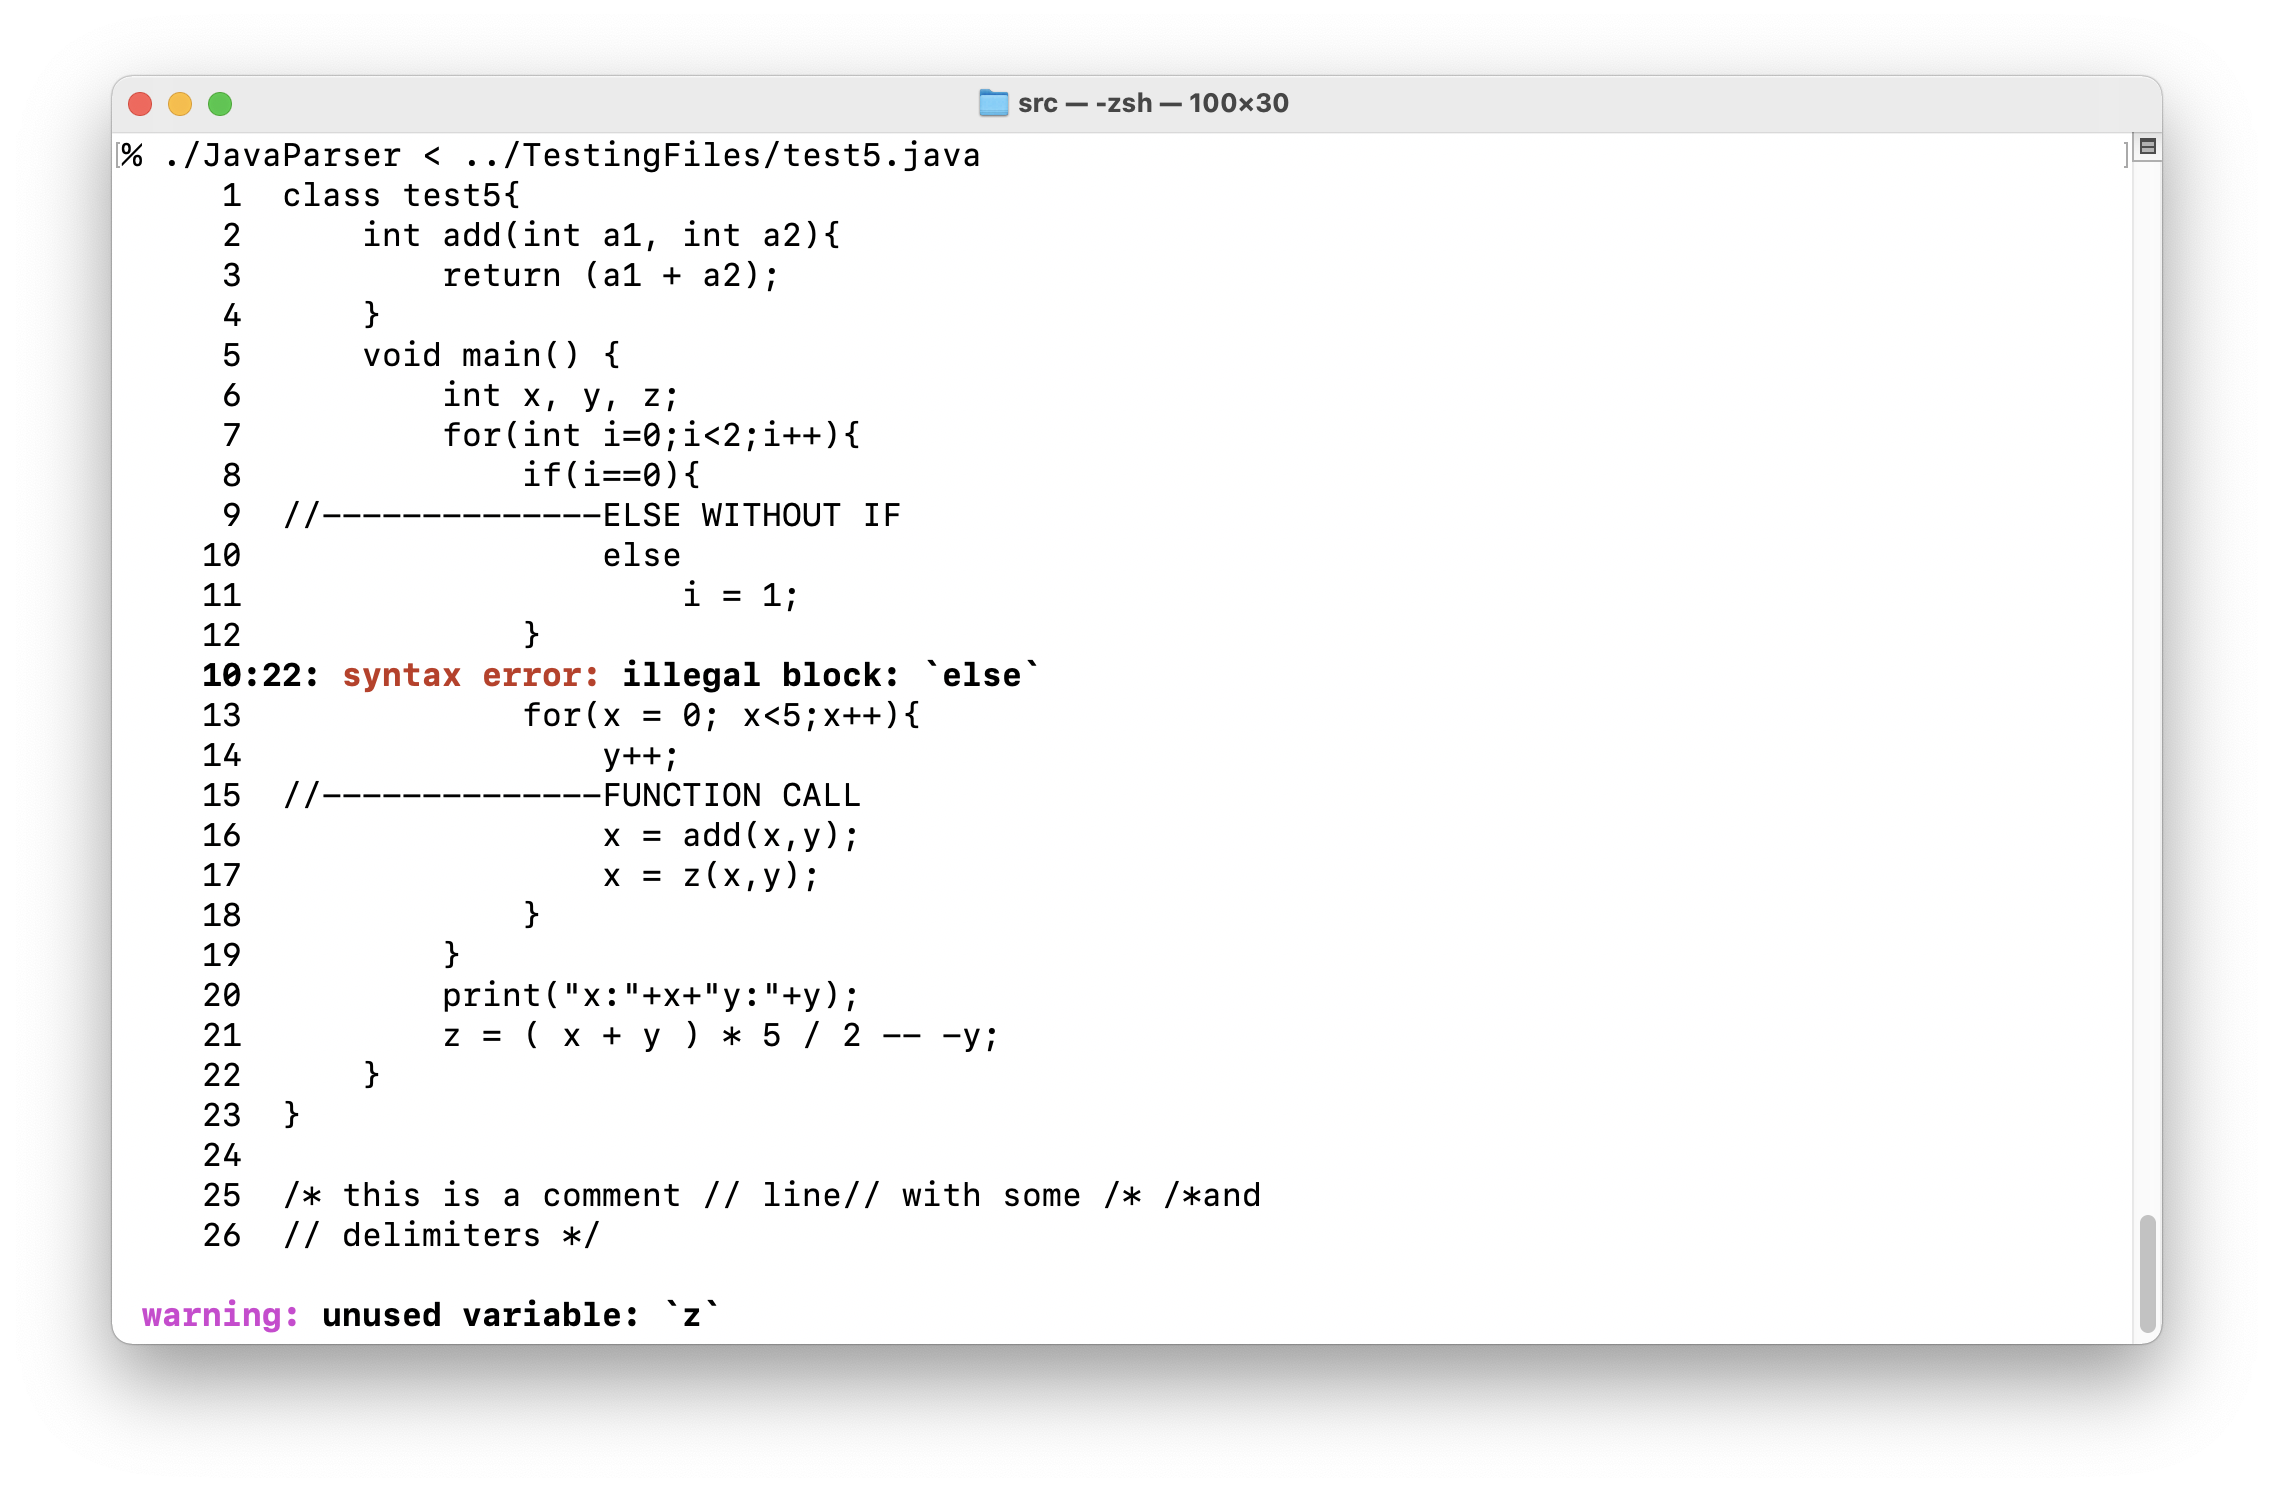
\includegraphics[width=0.9\textwidth]{Screenshots/test5}
\end{center}
\caption{The output of parsing \texttt{test5.java} with \texttt{DEBUG=1}}
\label{test1}
\end{figure}
\begin{figure}
\begin{center}
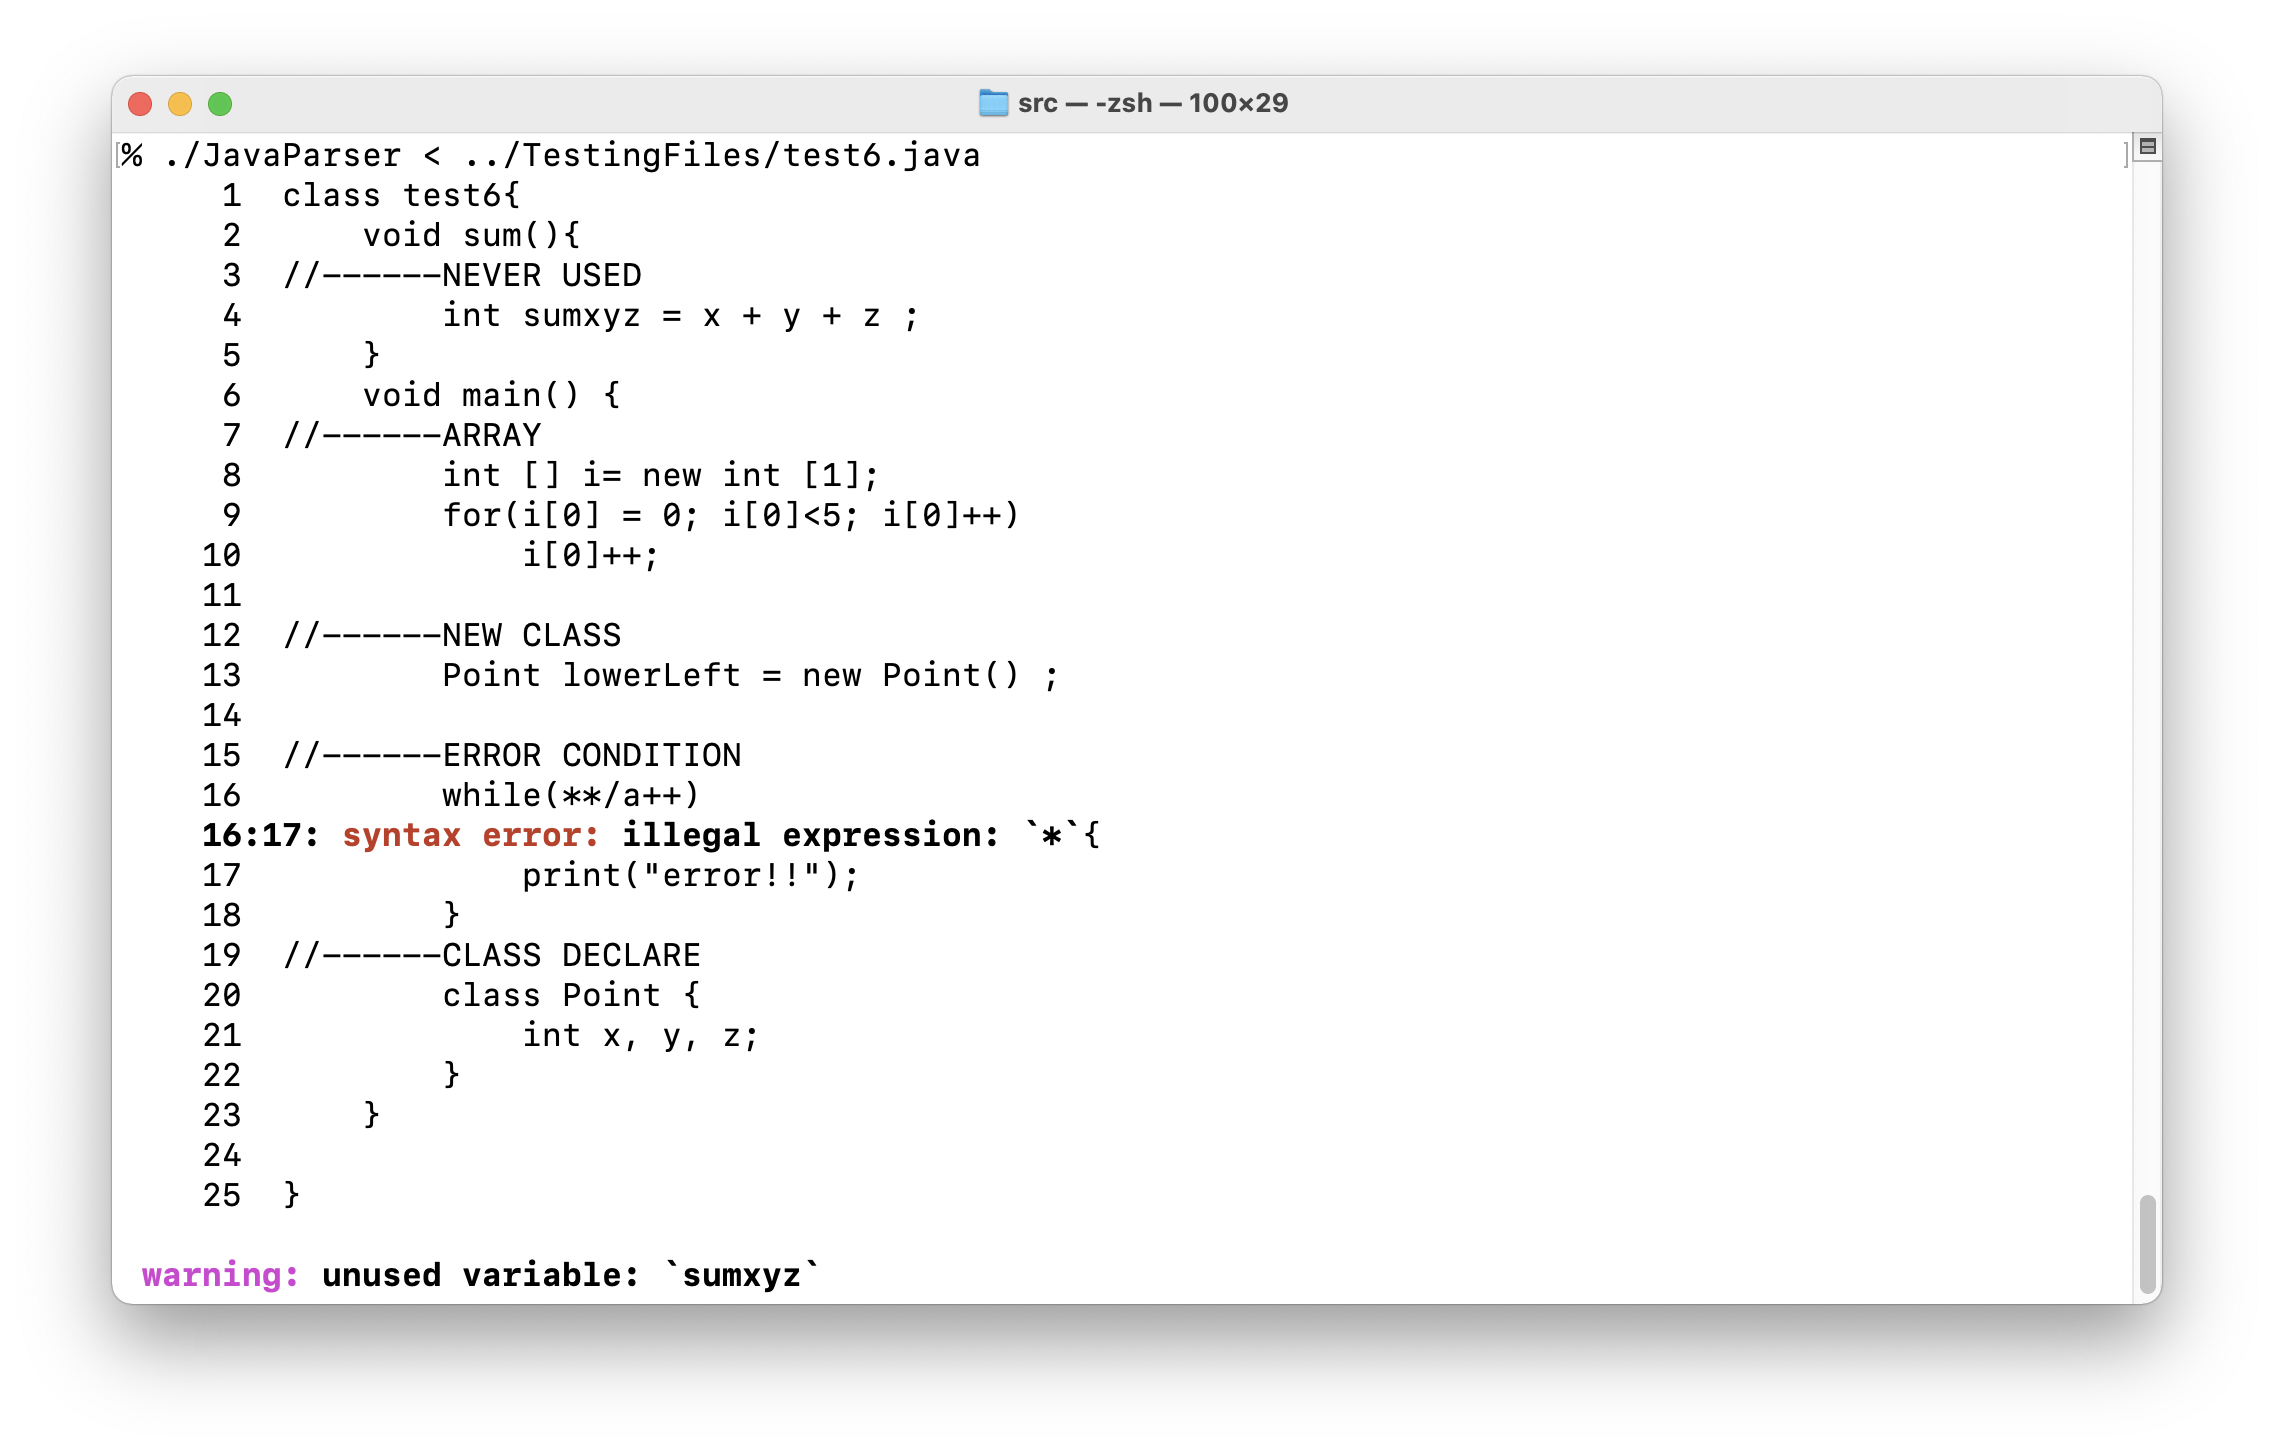
\includegraphics[width=0.9\textwidth]{Screenshots/test6}
\end{center}
\caption{The output of parsing \texttt{test6.java} with \texttt{DEBUG=1}}
\label{test1}
\end{figure}

\end{document}
